% !TEX program = pdflatex
% !TEX ext =  --interaction=nonstopmode --enable-etex --enable-write18
% !BIB program = biber
%%%==============================================================================
%% Copyright 2022-present by Alceu Frigeri
%%
%% Document (sample) file using the class ufrgscca
%%
%%%==============================================================================
\documentclass[repeatfields,xlists,xpacks,oneside]{ufrgscca}

\addbibresource{modeloTCC.bib}

\usepackage{float}
\usepackage{placeins}
\usepackage{tikz}
\usetikzlibrary{
    arrows.meta,
    positioning,
    calc
}

\usepackage{listings}
\usepackage{xcolor}
\usepackage{booktabs}  % MELHORIA: tabelas mais elegantes

% Define I2C como comando
\newcommand{\IIC}{I\textsuperscript{2}C}

% Estilo básico para os listings de código
\lstset{
  basicstyle=\ttfamily\small,
  breaklines=true,
  frame=single,
  numbers=left,
  numberstyle=\tiny,
  keywordstyle=\bfseries,
  commentstyle=\itshape\color{gray},
  inputencoding=utf8
}

\usepackage{float}

\newfloat{quadro}{htbp}{loq}
\floatname{quadro}{Quadro}
\newcommand{\fonte}[1]{\par\centering\footnotesize\textit{Fonte: #1}\par}

\begin{document}

\MakeCoverPages{tccI}

\notoc\chapter{Dedicatória}

Dedico este trabalho aos meus pais, em especial pela dedicação e apoio em
todos os momentos difíceis.

\notoc\chapter{Agradecimentos}

\`{A} Universidade Federal do Rio Grande do Sul, UFRGS, pela
oportunidade de realização de estudos.

Aos colegas de curso pelo seu auxílio nas tarefas desenvolvidas durante o
curso e apoio na revisão deste trabalho.

Agradeço ao \LaTeX\ por não ter vírus de macro\ldots


% palavras-chave
\mainkeywords{Engenharia Elétrica}
\mainkeywords{Processamento de Sinais}
\mainkeywords{Automação e Controle}
\mainkeywords{Eletrônica e Instrumentação}

\begin{mainabstract}

Este documento foi criado com o objetivo de auxiliar aos alunos
de graduação
da Universidade Federal do Rio Grande do Sul (UFRGS) no desenvolvimento dos
volumes finais de seus trabalhos de conclus\~{a}o de curso. O presente
documento serve, ao mesmo tempo, como modelo do formato de apresentação
oficial do TCC-CCA, bem como de roteiro para as etapas de elaboração do texto
técnico que o compõe. Os modelos e formatações aqui contidos são baseados em
normas da Associação Brasileira de Normas Técnicas (ABNT), em especial a
NBR-14724~\cite{ABNT:NBR-14724-2011}, que descreve o procedimento de elaboração e
apresentação de trabalhos acadêmicos (dissertações, teses, monografias,
entre outros).

\end{mainabstract}

\otherkeywords{Electrical Engineering}
\otherkeywords{Signal Processing}
\otherkeywords{Automation and Control}
\otherkeywords{Electronic and Instrumentation}

\begin{otherabstract}
This document aims to support undergraduated students  of Universidade Federal do Rio
Grande do Sul (UFRGS) in the development of their diplom project relatory.
This document serves concomitantly as a model of the official TCC-CCA
presentation layout as well as a guide throughout technical text composition
steps. The model and format held here are based in norms of the Associação
Brasileira de Normas Técnicas (ABNT), mainly in
NBR-14724~\cite{ABNT:NBR-14724-2011} which defines guidelines of design and
presentation of academic documents.
\end{otherabstract}


\setcounter{tocdepth}{3}

\listoffigures
\listoftables
\listofcodelist

% MELHORIA: lista de abreviaturas complementada com SHT20, PWM, HVAC, CSV, GUI
\begin{listofabbrv}{PPGEE}
    \item[CSV]   Comma-Separated Values
    \item[FIFO]  First In, First Out
    \item[GUI]   Graphical User Interface
    \item[HVAC]  Heating, Ventilation and Air Conditioning
    \item[ISR]   Interrupt Service Routine
    \item[PID]   Proporcional-Integral-Derivativo
    \item[PWM]   Pulse Width Modulation
    \item[RTOS]  Real Time Operating System
    \item[SHT20] Sensor de temperatura e umidade digital (Sensirion)
    \item[UART]  Universal Asynchronous Receiver-Transmitter
\end{listofabbrv}

\begin{listofsymbols}{$\alpha\beta\pi\omega$}
       \item[$\sum$] Somatório
       \item[$\alpha\beta\pi\omega$] Fator de inconstância do resultado
\end{listofsymbols}

\tableofcontents


% ============================================================
\chapter{Introdução}
% ============================================================

Nas últimas décadas, o avanço tecnológico na área de sistemas embarcados,
aliado ao crescimento da Internet das Coisas (IoT), tem impulsionado a demanda
por sistemas cada vez mais complexos e capazes de interagir de forma eficiente
com o mundo real. Dentro desse cenário, os sistemas de tempo real tornam-se essenciais,
pois a validade do sistema não está relacionada apenas à exatidão dos resultados obtidos,
mas também ao momento em que esses resultados são gerados~\cite{SPOHN:FreeRTOS-Arduino-2019}.
Vale ressaltar que não é obrigatório que a resposta a um evento ocorra no menor tempo possível,
sendo mais importante que os prazos definidos para cada tarefa sejam rigorosamente
atendidos~\cite{denardin2019rtos}. Essa característica garante um comportamento mais
determinístico do sistema, permitindo que as tarefas sejam concluídas dentro de prazos
previamente estabelecidos, mesmo diante de variações nas condições de execução. Caso essas
restrições temporais não sejam respeitadas, o sistema pode apresentar degradação de desempenho,
inconsistências operacionais ou até falhas críticas, especialmente em aplicações onde confiabilidade
e segurança são requisitos fundamentais.

Dentre as soluções de software disponíveis, o FreeRTOS~\cite{aws2024freertos} destaca-se como um kernel
de tempo real amplamente utilizado em microcontroladores devido à sua robustez,
modularidade e por ser um software de código aberto. Ele permite que a aplicação
seja organizada como um conjunto de tarefas independentes, onde um escalonador
decide qual tarefa deve ser executada com base em prioridades definidas pelo
projetista~\cite{barry2016freertos}. Esse modelo oferece vantagens em relação às
abordagens convencionais baseadas em laço principal (``superloop'' ou bare-metal),
que tendem a se tornar desorganizadas e menos eficientes à medida que a complexidade
do sistema aumenta. Em aplicações multitarefa, a disputa por recursos pode resultar
em atrasos indesejados e dificultar o controle adequado da execução das diferentes funções.

Para projetar e validar as estratégias de controle em sistemas dessa natureza, torna-se
indispensável o uso de ambientes de computação técnica, como o MATLAB~\cite{mathworks_matlab}. Essas plataformas
permitem não apenas a modelagem e a simulação do comportamento dinâmico de sistemas complexos,
mas também a integração direta com o hardware por meio do modo externo. Essa funcionalidade
viabiliza o monitoramento de variáveis em tempo real, facilitando a análise de desempenho e o
ajuste de parâmetros de controle diretamente no dispositivo embarcado, o que reduz o distanciamento
entre o modelo matemático e a execução física.

No contexto acadêmico e de pesquisa, essa integração é frequentemente explorada por meio de plantas
didáticas, que servem como elo entre a teoria de controle e a implementação prática. O controle de
temperatura, especificamente, representa uma aplicação clássica e de alta relevância industrial,
oferecendo dinâmicas ideais para validar a eficácia de algoritmos, como o PID, sob a gestão de um RTOS.
% MELHORIA: menção explícita à planta Quanser HVAC já na introdução
Neste trabalho, é utilizada uma planta didática baseada no módulo HVAC (\textit{Heating, Ventilation
and Air Conditioning}) da Quanser, adaptada para controle embarcado com o microcontrolador ATmega328P.
O uso de tal planta permite que desafios inerentes ao mundo real, como ruídos de sensores e latências
de processamento, sejam enfrentados e mitigados de forma controlada.

Diante desse cenário, este trabalho tem como objetivo desenvolver uma metodologia para o controle
em tempo real utilizando o FreeRTOS integrado ao ambiente MATLAB, aplicada à planta térmica
didática mencionada. A proposta busca não apenas validar a arquitetura de software desenvolvida, mas também
analisar de que forma o escalonamento de tarefas impacta o desempenho do processo. Com isso,
pretende-se consolidar um guia prático para a implementação de sistemas de controle multitarefa em
plataformas embarcadas, garantindo o rigor temporal e a eficiência operacional.

% MELHORIA: parágrafo de justificativa explícita
\section{Justificativa}

Apesar da ampla utilização do FreeRTOS em sistemas embarcados industriais, a literatura em
língua portuguesa ainda carece de trabalhos que integrem esse sistema operacional de tempo real
ao ambiente MATLAB de forma experimental e documentada. A maior parte das referências disponíveis
aborda o FreeRTOS de maneira isolada, sem contemplar o fluxo completo que vai desde a execução
multitarefa no microcontrolador até a supervisão e análise de dados em tempo real por uma interface
gráfica. Este trabalho busca preencher essa lacuna ao propor, implementar e validar uma arquitetura
que cubra todas essas etapas, utilizando hardware de baixo custo e ferramentas acessíveis no contexto
acadêmico da UFRGS. Os resultados obtidos poderão servir de referência para disciplinas de sistemas
embarcados, controle e automação, além de orientar projetos futuros que demandem integração entre
RTOS e ferramentas de supervisão.

\section{Objetivos}

\subsection{Objetivo Geral}

Desenvolver e validar uma arquitetura de controle em tempo real para sistemas embarcados, utilizando o sistema operacional FreeRTOS, com integração a ferramentas de supervisão e análise no ambiente MATLAB, visando aplicações em plantas didáticas.

\subsection{Objetivos Específicos}

\begin{itemize}
    \item Implementar e gerenciar tarefas concorrentes em um microcontrolador utilizando o FreeRTOS, considerando aspectos de escalonamento e temporização.

    \item Desenvolver e implementar algoritmos de controle adequados para execução em tempo real em sistemas embarcados.

    \item Integrar o sistema embarcado ao ambiente MATLAB para fins de monitoramento, aquisição de dados e análise do comportamento dinâmico.

    \item Validar experimentalmente a arquitetura proposta por meio de sua aplicação em uma planta térmica didática.

    \item Analisar a influência do escalonamento de tarefas no desempenho do sistema de controle.
\end{itemize}


% ============================================================
\chapter{Fundamentação Teórica}
\label{fundamentacao}
% ============================================================

Este capítulo estabelece os pilares teóricos necessários para a compreensão e o desenvolvimento do sistema de controle térmico sob um sistema operacional de tempo real. A fundamentação abrange desde a teoria de controle clássica até as especificidades arquiteturais do FreeRTOS e sua integração com ferramentas de computação técnica.

% ------------------------------------------------------------
\section{Sistemas em Malha Aberta e Malha Fechada}
% ------------------------------------------------------------

A classificação de sistemas de controle é fundamentada na topologia do fluxo de sinais. De acordo com Nise \citeyear{Nise2017}, sistemas em malha aberta são aqueles cuja ação de controle independe da saída do processo, conforme ilustrado na Figura \ref{fig:malha_aberta}. Embora apresentem baixa complexidade e custo reduzido, esses sistemas são incapazes de compensar perturbações externas ou variações nos parâmetros internos da planta.

Em contrapartida, sistemas em malha fechada utilizam o princípio da realimentação (\textit{feedback}). Segundo Ogata \citeyear{Ogata2010}, a malha fechada permite que a saída do sistema seja continuamente comparada a um valor de referência (\textit{setpoint}), como apresentado na Figura \ref{fig:malha_fechada}. O erro resultante dessa comparação orienta o controlador a ajustar a variável manipulada, conferindo ao sistema maior precisão, robustez e capacidade de rejeição a distúrbios, ainda que exija um projeto de estabilidade mais rigoroso para evitar oscilações indesejadas.

\begin{figure}[htbp]
    \centering
    \caption{Diagrama de um sistema em malha aberta}
    \label{fig:malha_aberta}
    \includegraphics[width=0.8\textwidth]{figuras/Malha Aberta.png}
    \caption*{\footnotesize Fonte: Autor.}
\end{figure}

\begin{figure}[htbp]
    \centering
    \caption{Diagrama de um sistema em malha fechada}
    \label{fig:malha_fechada}
    \includegraphics[width=0.8\textwidth]{figuras/Malha Fechada.png}
    \caption*{\footnotesize Fonte: Autor.}
\end{figure}

% ------------------------------------------------------------
\section{Estratégias de Controle}
% ------------------------------------------------------------

\subsection{Controlador PID}

O controlador Proporcional-Integral-Derivativo (PID) é uma das estratégias de controle mais utilizadas na automação industrial devido à sua simplicidade de implementação e elevada eficiência em diferentes tipos de processos. Segundo Júnior e Silva \citeyear{Junior2015}, a ampla aplicação desse controlador está associada à sua capacidade de conduzir o sistema ao ponto de operação desejado de maneira rápida, reduzindo oscilações e minimizando o erro em regime permanente.

A ação de controle do PID é composta por três parcelas fundamentais:

\begin{itemize}
    \item \textbf{Proporcional ($K_p$):} produz uma ação proporcional ao erro instantâneo, proporcionando resposta rápida às variações do sistema;

    \item \textbf{Integral ($K_i$):} acumula o erro ao longo do tempo, atuando na eliminação do erro em regime permanente;

    \item \textbf{Derivativo ($K_d$):} considera a taxa de variação do erro, antecipando tendências e contribuindo para o amortecimento da resposta do sistema.
\end{itemize}

Matematicamente, a ação de controle de um controlador PID pode ser descrita por:

\begin{equation}
    u(t) = K_p e(t) + K_i \int_0^t e(\tau)\, d\tau + K_d \frac{de(t)}{dt}
\end{equation}

Uma forma alternativa, também amplamente empregada na literatura e em aplicações industriais, é apresentada pela Equação \ref{formula:pid} \cite{Bazanella2005}:

\begin{equation}
    u(t) = K \left( e(t) + \frac{1}{T_i} \int_0^t e(\tau)\, d\tau + T_d \frac{de(t)}{dt} \right)
    \label{formula:pid}
\end{equation}

Nessa representação, $K$ corresponde ao ganho proporcional do controlador, $T_i$ representa a constante de tempo associada à ação integral e $T_d$ a constante de tempo da ação derivativa. O termo $e(t)$ representa o erro entre o valor de referência e a saída do sistema. A adequada combinação desses parâmetros permite ajustar características importantes da resposta dinâmica, como tempo de subida, sobressinal, tempo de acomodação e erro em regime permanente.

Na prática, a sintonia dos parâmetros do controlador pode ser realizada por diferentes abordagens, desde métodos empíricos, como o método de Ziegler-Nichols, até técnicas analíticas e computacionais mais avançadas, dependendo da complexidade e das exigências do sistema. Um ajuste inadequado desses parâmetros pode resultar em oscilações excessivas, respostas lentas ou até mesmo instabilidade.

% MELHORIA: PID discreto — equação de diferenças para implementação embarcada
\subsubsection{Implementação Discreta do Controlador PID}

Em sistemas embarcados, o controlador PID é necessariamente implementado de forma discreta, pois o microcontrolador opera sobre amostras periódicas do sinal de erro. Adotando a aproximação de Euler regressivo (diferenças atrasadas) com período de amostragem $T$, as integrais e derivadas contínuas são substituídas por:

\begin{equation}
    \int_0^t e(\tau)\,d\tau \;\approx\; T \sum_{k=0}^{n} e[k]
    \qquad\text{e}\qquad
    \frac{de(t)}{dt} \;\approx\; \frac{e[n] - e[n-1]}{T}
\end{equation}

A equação de diferenças resultante, em sua forma posicional, é:

\begin{equation}
    u[n] = K\!\left( e[n]
           + \frac{T}{T_i}\sum_{k=0}^{n} e[k]
           + \frac{T_d}{T}\bigl(e[n]-e[n-1]\bigr) \right)
    \label{eq:pid_discreto}
\end{equation}

Na forma incremental (também chamada de forma de velocidade), calcula-se apenas a variação do sinal de controle a cada instante, o que facilita o tratamento de saturação (\textit{anti-windup}) e a troca bumpless entre modos de operação:

\begin{equation}
    \Delta u[n] = u[n] - u[n-1]
               = K\!\left(
                   e[n] - e[n-1]
                 + \frac{T}{T_i}\,e[n]
                 + \frac{T_d}{T}\bigl(e[n] - 2e[n-1] + e[n-2]\bigr)
                 \right)
    \label{eq:pid_incremental}
\end{equation}

A Equação~\ref{eq:pid_discreto} será a base da implementação na \texttt{TaskControl}, descrita no Capítulo~\ref{cap:metodologia}. Para mitigar o efeito de ruído de medição amplificado pela ação derivativa, será adotado um filtro de primeira ordem com polo $p$ sobre o termo derivativo, conforme parametrizado na interface gráfica (Tabela~\ref{tab:gui_params}).

A Figura \ref{fig:pid_diagrama} apresenta a estrutura típica de um controlador PID baseado na representação mostrada na Equação \ref{formula:pid}, aplicada a um sistema de controle em malha fechada.

\begin{figure}[htbp]
    \centering
    \caption{Diagrama de um sistema de controle com controlador PID}
    \label{fig:pid_diagrama}
    \includegraphics[width=0.8\textwidth]{figuras/diagrama PID.png}
    \caption*{\footnotesize Fonte: \cite{Bazanella2005}.}
\end{figure}

\subsection{Controle Liga-Desliga (Bang-Bang)}

Comum em sistemas de climatização e aquecimento simples, o controle liga-desliga opera de forma binária. O atuador é ativado ou desativado com base no sinal do erro, sem níveis intermediários de atuação. Esse tipo de estratégia é conhecido como controle de dois níveis ou \textit{on-off control}, sendo amplamente utilizado devido à sua simplicidade e baixo custo \cite{Ogata2010}.

Nesse contexto, a ação bang-bang corresponde a um controlador cujo sinal de saída assume apenas dois valores distintos, conforme descrito por Bazanella e Gomes da Silva Jr. \citeyear{Bazanella2005}. A lei de controle pode ser expressa de forma simplificada como:

\begin{equation}
    u(t) =
    \begin{cases}
        U_{\text{max}}, & \text{se } e(t) > 0 \\
        U_{\text{min}}, & \text{se } e(t) < 0
    \end{cases}
\end{equation}

onde $e(t)$ representa o erro entre o valor de referência e a variável de processo. Devido à natureza discreta da ação de controle, o sistema tende a apresentar oscilações em torno do \textit{setpoint}, caracterizando um comportamento típico de ciclo limite \cite{Ogata2010}.

Uma forma comum de mitigar o efeito de chaveamento excessivo é a introdução de uma banda de histerese, criando uma região de tolerância em torno do \textit{setpoint}. Essa abordagem reduz a frequência de comutação e evita chaveamentos indesejados na presença de ruído \cite{Bazanella2005}.

Apesar de suas limitações em termos de precisão e desempenho dinâmico, o controle liga-desliga permanece amplamente utilizado em aplicações onde pequenas oscilações são aceitáveis e a simplicidade é um fator determinante \cite{Ogata2010}.

A Figura \ref{fig:bangbang} ilustra o comportamento típico de um controlador liga-desliga aplicado a um sistema de controle.

\begin{figure}[htbp]
    \centering
    \caption{Diagrama de um sistema com controle liga-desliga (bang-bang)}
    \label{fig:bangbang}
    \includegraphics[width=0.8\textwidth]{figuras/diagrama BangBang.png}
    \caption*{\footnotesize Fonte: \cite{Bazanella2005}.}
\end{figure}

% ------------------------------------------------------------
\section{Sistemas Operacionais de Tempo Real (RTOS)}
% ------------------------------------------------------------

Diferentemente dos sistemas operacionais de propósito geral, cujo objetivo principal é maximizar o desempenho médio e a interação com o usuário, um Sistema Operacional de Tempo Real (RTOS) é projetado para garantir previsibilidade temporal. Isso implica que não basta apenas que os resultados estejam logicamente corretos, mas que também sejam produzidos dentro de intervalos de tempo previamente estabelecidos. Conforme Laplante \citeyear{Laplante2004}, a validade de um sistema de tempo real depende diretamente do cumprimento rigoroso dos prazos (\textit{deadlines}), sendo que uma resposta correta fora do tempo especificado pode ser considerada inválida.

Os sistemas de tempo real podem ser classificados quanto à rigidez de seus requisitos temporais em três categorias \cite{SPOHN:FreeRTOS-Arduino-2019}:

\begin{itemize}
    \item \textbf{\textit{Hard}:} o não cumprimento dos prazos inutiliza completamente o sistema;

    \item \textbf{\textit{Firm}:} o resultado fora do prazo torna-se inútil, mas não compromete o sistema como um todo;

    \item \textbf{\textit{Soft}:} o descumprimento dos prazos impacta apenas o desempenho, sem causar dano grave.
\end{itemize}

Nesse contexto, o RTOS oferece mecanismos essenciais para o desenvolvimento de aplicações críticas, como o gerenciamento de múltiplas tarefas concorrentes, sincronização entre processos e controle preciso de temporização. Denardin e Barriquello \citeyear{denardin2019rtos} ressaltam que o uso de um RTOS permite organizar a aplicação em tarefas independentes, cada uma responsável por uma funcionalidade específica, como aquisição de dados de sensores, execução de algoritmos de controle ou comunicação com outros dispositivos. Essas tarefas são gerenciadas por um escalonador (\textit{scheduler}), que determina qual tarefa deve ser executada a cada instante com base em critérios como prioridade e tempo de execução.

Dessa forma, o uso de um RTOS garante que requisitos fundamentais --- como a manutenção de uma taxa de amostragem constante da planta térmica --- sejam atendidos, contribuindo diretamente para a estabilidade e o desempenho do sistema de controle.

% ------------------------------------------------------------
\section{FreeRTOS e Microcontroladores}
% ------------------------------------------------------------

O FreeRTOS é um sistema operacional de tempo real de código aberto, desenvolvido em linguagem C e projetado para aplicações embarcadas que demandam previsibilidade temporal e execução multitarefa em ambientes com recursos restritos \cite{barry2016freertos}. No contexto do microcontrolador ATmega328P, o FreeRTOS substitui o modelo tradicional de laço único (\textit{superloop}) por um núcleo (\textit{kernel}) que gerencia tarefas independentes, conferindo maior modularidade e escalabilidade ao projeto \cite{SPOHN:FreeRTOS-Arduino-2019}.

% MELHORIA: tabela de parâmetros relevantes do ATmega328P
\subsection{Características Relevantes do ATmega328P}

A Tabela~\ref{tab:atmega_params} reúne os principais parâmetros do microcontrolador ATmega328P
relevantes para a implementação do sistema proposto, consolidando informações que são referenciadas
ao longo dos capítulos seguintes.

\begin{table}[htbp]
\centering
\caption{Parâmetros relevantes do microcontrolador ATmega328P.}
\label{tab:atmega_params}
\begin{tabular}{lll}
\toprule
\textbf{Parâmetro} & \textbf{Valor} & \textbf{Observação} \\
\midrule
Frequência de clock     & 16\,MHz       & Arduino Nano/Uno \\
Memória SRAM            & 2\,KB         & Compartilhada entre pilhas e heap \\
Memória Flash           & 32\,KB        & Código + dados do FreeRTOS \\
EEPROM                  & 1\,KB         & Armazenamento não volátil \\
Timers de 8 bits        & 2 (Timer0, Timer2) & PWM de até 8 bits \\
Timer de 16 bits        & 1 (Timer1)    & PWM de até 10 bits / base de tempo RTOS \\
Canais PWM              & 6             & Pinos D3, D5, D6, D9, D10, D11 \\
Barramento \IIC{}       & 1             & Pinos A4 (SDA) e A5 (SCL) \\
UART                    & 1             & Pinos D0 (RX) e D1 (TX) \\
\bottomrule
\end{tabular}
\caption*{\footnotesize Fonte: Autor, com base no \textit{datasheet} do ATmega328P \cite{atmel_atmega328p}.}
\end{table}

\subsection{Gerenciamento de Tarefas e Estados}

No FreeRTOS, as aplicações são organizadas como coleções de tarefas independentes, semelhantes a \textit{threads}, cada uma possuindo sua própria pilha (\textit{stack}) e um bloco de controle denominado \textit{Task Control Block} (TCB) \cite{SPOHN:FreeRTOS-Arduino-2019}. Em processadores de núcleo único, como o ATmega328P, o escalonador promove uma rápida alternância entre tarefas, criando a ilusão de simultaneidade (\textit{pseudo-paralelismo}).

O bloco de controle de tarefa (\textit{Task Control Block} -- TCB) armazena as informações necessárias para o gerenciamento de cada tarefa pelo escalonador do sistema operacional. Entre essas informações estão o ponteiro da pilha da tarefa, registradores salvos durante trocas de contexto, estado atual da tarefa e nível de prioridade. Conforme descrito por Denardin e Barriquello \citeyear{denardin2019rtos}, o TCB é essencial para que o RTOS consiga interromper e restaurar tarefas de forma transparente durante o escalonamento.

A Figura \ref{fig:tcb_tasks} apresenta uma representação simplificada da organização das tarefas em memória, destacando a relação entre as pilhas individuais, os TCBs e o processador.

\begin{figure}[htbp]
    \centering
    \caption{Estrutura de múltiplas tarefas compartilhando o processador.}
    \label{fig:tcb_tasks}
    \includegraphics[width=0.6\textwidth]{figuras/tcb_tasks.png}
    \caption*{\footnotesize Fonte: \cite{denardin2019rtos}.}
\end{figure}

As tarefas transitam entre diferentes estados de execução ao longo do funcionamento do sistema operacional. Os principais estados utilizados no FreeRTOS são:

\begin{itemize}
    \item \textbf{Executando:} a tarefa está utilizando o processador naquele instante;

    \item \textbf{Pronta:} a tarefa está apta para execução, aguardando apenas a liberação da CPU pelo escalonador;

    \item \textbf{Bloqueada:} a tarefa aguarda um evento temporal ou de sincronização, como atraso periódico, recebimento de mensagem em fila ou liberação de semáforo;

    \item \textbf{Suspensa:} a tarefa foi removida explicitamente do escalonador, retornando apenas mediante chamada específica da API do FreeRTOS.
\end{itemize}

A Figura \ref{fig:estados_tarefas} ilustra os estados fundamentais das tarefas e as possíveis transições entre eles em um sistema multitarefa.

\begin{figure}[htbp]
    \centering
    \caption{Estados das tarefas em um sistema multitarefa.}
    \label{fig:estados_tarefas}
    \includegraphics[width=0.85\textwidth]{figuras/estados_tarefas.png}
    \caption*{\footnotesize Fonte: \cite{denardin2019rtos}.}
\end{figure}

Durante a troca de contexto, o estado da tarefa atualmente em execução é salvo em sua pilha e no respectivo TCB, permitindo que outra tarefa utilize o processador. Quando a tarefa interrompida retorna à execução, seu contexto anterior é restaurado, garantindo continuidade transparente da aplicação \cite{denardin2019rtos}.

\subsection{Mecanismos de Escalonamento}

O escalonador decide qual tarefa utilizará a CPU com base em prioridades fixas definidas pelo desenvolvedor. Conforme Spohn, Neto e Fassini \citeyear{SPOHN:FreeRTOS-Arduino-2019}, o sistema opera em dois modos principais:

\begin{itemize}
    \item \textbf{Escalonamento preemptivo:} se uma tarefa de maior prioridade tornar-se pronta, ela interrompe imediatamente a tarefa atual (\textit{troca de contexto}), reduzindo a latência e assegurando o determinismo exigido em sistemas de controle. Testes realizados na plataforma Arduino Uno demonstraram latência média de troca de contexto de apenas 7,74\,µs \cite{SPOHN:FreeRTOS-Arduino-2019};

    \item \textbf{Fatiamento de tempo (\textit{time slicing}):} utiliza interrupções periódicas do sistema (\textit{ticks}) para compartilhar o processador equitativamente entre tarefas de mesma prioridade.
\end{itemize}

Embora os testes reportados por Spohn, Neto e Fassini \citeyear{SPOHN:FreeRTOS-Arduino-2019} tenham sido realizados na plataforma Arduino Uno, os resultados são diretamente aplicáveis ao Arduino Nano utilizado neste trabalho, uma vez que ambas as plataformas utilizam o mesmo microcontrolador ATmega328P, operando à mesma frequência de clock de 16\,MHz.

\subsection{Jitter Temporal e Determinismo}

Em sistemas de controle em tempo real, pequenas variações no instante de execução das tarefas periódicas são conhecidas como \textit{jitter} temporal. Esse fenômeno ocorre devido a atrasos introduzidos pelo escalonador, interrupções concorrentes ou variações no tempo de execução das tarefas, podendo comprometer diretamente o desempenho de sistemas de controle digital.

Em aplicações embarcadas de controle, a manutenção de uma taxa de amostragem constante é fundamental para garantir estabilidade e previsibilidade da resposta dinâmica. Variações excessivas no período de amostragem podem alterar o comportamento do controlador discreto, produzindo oscilações indesejadas, degradação de desempenho ou até instabilidade do sistema.

Nesse contexto, o FreeRTOS oferece mecanismos para reduzir o \textit{jitter} e aumentar o determinismo temporal da aplicação. Uma das principais estratégias consiste na utilização da função \texttt{vTaskDelayUntil()}, que permite a execução periódica de tarefas com base em referências absolutas de tempo, minimizando o acúmulo de atrasos ao longo das execuções sucessivas.

Além disso, o escalonamento preemptivo baseado em prioridades garante que tarefas críticas, como aquisição de sensores e execução do algoritmo de controle, tenham acesso prioritário ao processador sempre que necessário. Essa característica contribui diretamente para o comportamento determinístico exigido em aplicações de controle em tempo real.

\subsection{Timers, Interrupções e Controle de Recursos}

O FreeRTOS disponibiliza \textit{timers} de software para agendamento de ações periódicas ou temporizadas sob controle do kernel, operando no modo \textit{one-shot} (executado uma única vez) ou \textit{auto-reload} (reiniciado automaticamente a cada período) \cite{SPOHN:FreeRTOS-Arduino-2019}. As rotinas de interrupção (\textit{Interrupt Service Routines} -- ISR) possuem prioridade superior às tarefas convencionais, garantindo menor latência no tratamento de eventos críticos; recomenda-se, contudo, que executem apenas operações rápidas, delegando o processamento mais complexo a tarefas do sistema.

\subsection{Comunicação e Sincronização entre Tarefas}

Em ambientes multitarefa, tarefas compartilham a memória global do sistema sem proteção automática, o que torna possível que uma tarefa seja interrompida durante a escrita de uma variável compartilhada por outra de maior prioridade. Esse cenário caracteriza as chamadas condições de corrida (\textit{race conditions}), podendo gerar corrupção de dados e comportamentos não determinísticos --- problema especialmente crítico em aplicações de controle em tempo real \cite{denardin2019rtos}.

Para prevenir tais situações, o FreeRTOS oferece um conjunto de mecanismos de comunicação e sincronização entre tarefas (\textit{Interprocess Communication} -- IPC) \cite{barry2016freertos}:

\begin{itemize}
    \item \textbf{Filas (\textit{Queues}):} estruturas FIFO utilizadas para envio seguro de dados entre tarefas ou entre rotinas de interrupção e tarefas;

    \item \textbf{Semáforo Binário:} mecanismo de sincronização entre duas tarefas ou de sinalização de eventos simples;

    \item \textbf{Semáforo Contador (\textit{Counting Semaphore}):} extensão do semáforo binário que possibilita controlar múltiplas ocorrências simultâneas de um mesmo recurso compartilhado;

    \item \textbf{MUTEX (\textit{Mutual Exclusion}):} mecanismo de exclusão mútua para proteção de regiões críticas. Diferentemente dos semáforos binários, implementa herança de prioridade, mitigando problemas de inversão de prioridade em sistemas multitarefa;

    \item \textbf{Notificações de Tarefa (\textit{Task Notifications}):} mecanismo leve de sinalização implementado diretamente no TCB da tarefa, dispensando estruturas auxiliares e reduzindo o overhead de comunicação.
\end{itemize}

\subsection{Restrições de Memória no ATmega328P}

A implementação do FreeRTOS no ATmega328P exige atenção rigorosa aos 2\,KB de SRAM disponíveis (ver Tabela~\ref{tab:atmega_params}). Conforme Spohn, Neto e Fassini \citeyear{SPOHN:FreeRTOS-Arduino-2019}, o \textit{port} para a arquitetura AVR utiliza o esquema \textbf{Heap 3}, que encapsula as funções \texttt{malloc()} e \texttt{free()} da biblioteca padrão; para garantir a segurança em ambiente multitarefa (\textit{thread-safety}), o kernel suspende temporariamente o escalonador durante as alocações. Como a pilha de cada tarefa é alocada na SRAM, pilhas excessivamente grandes ou um número elevado de tarefas podem causar colisão de memória (\textit{heap overflow}), resultando em instabilidades. Os testes mostram que é possível executar até 10 tarefas simultâneas, com pilhas de no máximo 89\,bytes cada.

\subsection{Integração e Robustez no Controle}

O FreeRTOS atua como uma camada de abstração entre o hardware e a aplicação, permitindo que diferentes funcionalidades do sistema sejam organizadas em tarefas independentes e executadas de forma concorrente \cite{Morais2018}. Essa arquitetura favorece a modularidade do software, simplifica a manutenção do código e melhora a escalabilidade da aplicação embarcada.

No sistema desenvolvido neste trabalho, tarefas críticas --- como aquisição do sensor de temperatura e execução do algoritmo de controle --- possuem prioridade elevada, garantindo previsibilidade temporal e baixa latência de resposta. Em contrapartida, tarefas de menor criticidade, como transmissão serial de dados ao MATLAB, são executadas com prioridade reduzida, evitando interferência direta sobre o laço de controle.

A utilização do FreeRTOS também contribui para o aumento da robustez do sistema, uma vez que o isolamento funcional das tarefas reduz o impacto de falhas locais sobre toda a aplicação. Além disso, mecanismos de sincronização, gerenciamento de memória e controle de prioridades permitem maior confiabilidade na execução simultânea de múltiplas funções em sistemas embarcados de recursos limitados.

% ------------------------------------------------------------
\section{Sensor SHT20 e Protocolo \IIC{}}
% ------------------------------------------------------------
% MELHORIA: subseção nova — sensor e I2C sem embasamento no original

O sensor SHT20 é um dispositivo digital de temperatura e umidade relativa desenvolvido pela Sensirion, amplamente utilizado em sistemas embarcados que demandam medições precisas e de baixo consumo energético. Suas principais características são a faixa de medição de temperatura entre $-40\,°C$ e $+125\,°C$, com precisão típica de $\pm 0{,}3\,°C$, e tempo de conversão configurável entre 14\,ms (resolução de 14 bits) e 85\,ms (resolução de 12 bits) \cite{sensirion_sht20}.

A comunicação com o sensor é realizada pelo protocolo \IIC{} (\textit{Inter-Integrated Circuit}), um barramento serial síncrono de dois fios criado pela Philips Semiconductors e descrito em \cite{nxp_i2c}. O protocolo utiliza duas linhas: SDA (\textit{Serial Data}) para transmissão dos dados e SCL (\textit{Serial Clock}) para o sinal de temporização. No ATmega328P, essas linhas correspondem, respectivamente, aos pinos A4 e A5.

O barramento \IIC{} opera com topologia mestre-escravo. O Arduino Nano atua como mestre, iniciando e encerrando cada transação, enquanto o SHT20 responde como escravo no endereço fixo \texttt{0x40}. Uma leitura típica de temperatura envolve as seguintes etapas:

\begin{enumerate}
    \item O mestre envia uma condição de início (\textit{START}) seguida do endereço do escravo e do bit de escrita;
    \item O mestre envia o comando de medição de temperatura (\texttt{0xF3} para modo sem \textit{hold} do mestre);
    \item Após o tempo de conversão, o mestre reinicia a comunicação e lê os dois bytes de resultado mais o byte de CRC;
    \item O valor bruto é convertido para graus Celsius pela equação: $T\,[\text{°C}] = -46{,}85 + 175{,}72 \cdot \frac{S_{T}}{2^{16}}$, onde $S_T$ é o valor bruto lido.
\end{enumerate}

No sistema desenvolvido, a biblioteca \texttt{SHT2x} é utilizada para abstrair o protocolo de comunicação, e a aquisição do sensor é realizada exclusivamente pela \texttt{TaskSensor}, eliminando acessos concorrentes ao barramento \IIC{}.

% ------------------------------------------------------------
\section{Modulação por Largura de Pulso (PWM) no ATmega328P}
% ------------------------------------------------------------
% MELHORIA: subseção nova — PWM sem embasamento no original

A Modulação por Largura de Pulso (PWM, do inglês \textit{Pulse Width Modulation}) é a técnica utilizada para controlar a potência entregue aos atuadores da planta térmica: a lâmpada de aquecimento e o cooler de ventilação. Na PWM, um sinal digital periódico alterna entre os níveis lógico alto e baixo; a relação entre o tempo em nível alto e o período total é denominada ciclo de trabalho (\textit{duty cycle}, $\delta$), variando de $0\,\%$ (atuador desligado) a $100\,\%$ (atuador na potência máxima).

O ATmega328P dispõe de três módulos de timer/contador que geram sinais PWM em hardware: Timer0 (8 bits), Timer1 (16 bits) e Timer2 (8 bits), totalizando seis canais PWM distribuídos nos pinos D3, D5, D6, D9, D10 e D11. A frequência da PWM depende da frequência de clock e do prescaler configurado; para os timers de 8 bits com prescaler de 64, a frequência resultante é:

\begin{equation}
    f_{PWM} = \frac{f_{clk}}{N \cdot 2^n}
            = \frac{16\times10^6}{64 \cdot 256}
            \approx 976\,\text{Hz}
\end{equation}

onde $N$ é o fator de prescaler e $n$ é a resolução em bits do timer. No Arduino, a função \texttt{analogWrite(pino, valor)} configura automaticamente o respectivo timer no modo PWM com resolução de 8 bits (0 a 255), sendo esse o mecanismo empregado no sistema para o controle da potência dos atuadores.

Ressalta-se que o Timer1, utilizado internamente pelo FreeRTOS como base de tempo para o \textit{tick} do kernel, não deve ser reconfigurado pela aplicação. Os canais de PWM associados à lâmpada e ao cooler utilizam, portanto, o Timer0 (pinos D5 e D6) e o Timer2 (pinos D9 e D10), mantendo o Timer1 reservado ao kernel do sistema operacional.

% ------------------------------------------------------------
\section{Integração entre Arduino e Ambiente MATLAB}
% ------------------------------------------------------------

A integração entre sistemas embarcados e ambientes de computação técnica representa
uma abordagem consolidada no desenvolvimento e na validação de sistemas de controle,
tanto em contextos acadêmicos quanto industriais. Plataformas como o MATLAB
\cite{mathworks_matlab} oferecem recursos para modelagem, simulação, aquisição de dados
e análise do comportamento dinâmico de processos, complementando a execução
embarcada ao fornecer uma camada de supervisão externa ao microcontrolador.

Neste trabalho, será utilizada a plataforma MATLAB R2014a, disponibilizada por meio
da licença institucional da Universidade Federal do Rio Grande do Sul (UFRGS). A escolha
dessa versão deve-se à sua disponibilidade institucional, estabilidade de operação e ampla
compatibilidade com bibliotecas de comunicação serial utilizadas em sistemas embarcados.

Será desenvolvida uma Interface Gráfica do Usuário (GUI -- \textit{Graphical User Interface})
em ambiente MATLAB, destinada à supervisão e interação com a planta térmica controlada
por um microcontrolador Arduino Nano. A interface permitirá a comunicação serial
bidirecional entre o computador e o sistema embarcado, possibilitando o envio e o
recebimento de parâmetros em tempo real.

Nesse arranjo, o Arduino Nano será responsável pela execução das tarefas de controle
em tempo real, incluindo a aquisição dos sinais provenientes dos sensores, o cálculo das
ações de controle e o acionamento dos atuadores presentes na planta térmica. Por outro
lado, o MATLAB atuará como supervisório, realizando o monitoramento contínuo das
variáveis do processo e permitindo a alteração dinâmica dos parâmetros de operação sem
a necessidade de recompilação ou reinicialização do firmware.

A GUI desenvolvida possibilitará a visualização gráfica das variáveis do sistema, como
temperatura medida, sinal de controle aplicado e valor de referência, além da seleção dos
modos de operação da planta, incluindo estratégias de controle em malha aberta,
Bang-Bang e PID\@. Também serão disponibilizados campos para parametrização dos ganhos
de controle e indicadores numéricos referentes ao estado atual do sistema.

A comunicação entre os dois ambientes será estabelecida por meio de uma interface
serial UART, devido à sua simplicidade de implementação e ampla compatibilidade com
diferentes plataformas de hardware e software. O protocolo de
comunicação será baseado em mensagens textuais estruturadas no formato CSV
(\textit{Comma-Separated Values}), permitindo a troca bidirecional de informações de maneira
simples e eficiente. Nesse modelo, o Arduino Nano enviará continuamente os dados
monitorados da planta térmica ao MATLAB, enquanto a GUI poderá transmitir novos
parâmetros e comandos operacionais em tempo real.

No contexto de plantas didáticas, essa integração apresenta elevada relevância, pois
permite que fenômenos inerentes ao ambiente físico --- como ruídos de medição, atrasos
de comunicação, saturação de atuadores e variações paramétricas --- sejam observados e
analisados diretamente durante a execução experimental. Dessa forma, a utilização da GUI
supervisória em conjunto com o sistema embarcado contribui significativamente para a
validação prática das estratégias de controle implementadas e para o processo de
aprendizagem associado aos sistemas de controle embarcados.


% ============================================================
\chapter{Metodologia}
\label{cap:metodologia}
% ============================================================

\section{Descrição da Planta Térmica Didática}

A planta térmica didática utilizada neste trabalho é baseada no módulo HVAC (\textit{Heating, Ventilation and Air Conditioning}) da Quanser, adaptado para aplicações de controle embarcado com microcontrolador ATmega328. O sistema tem como objetivo permitir a implementação, validação e análise de diferentes estratégias de controle térmico em tempo real, integrando hardware embarcado, supervisão computacional e algoritmos de controle.

A estrutura física da planta é composta por uma fonte de aquecimento, responsável pela elevação da temperatura interna, e por um sistema de ventilação forçada, utilizado para promover o resfriamento do ambiente controlado. A variável de processo monitorada corresponde à temperatura interna, medida por sensor digital, enquanto as variáveis manipuladas são os sinais de acionamento dos atuadores de aquecimento e ventilação.

A Figura~\ref{fig:planta_real} apresenta uma visão geral da planta física.

\begin{figure}[htbp]
    \centering
    \includegraphics[width=0.40\textwidth, angle=90]{figuras/planta.jpeg}
    \caption{Vista geral da planta térmica didática HVAC utilizada nos experimentos.}
    \label{fig:planta_real}
    \caption*{\footnotesize Fonte: Autor.}
\end{figure}

\subsection{Arquitetura de Hardware e Componentes Utilizados}

O sistema é centrado no microcontrolador ATmega328P presente
no Arduino Nano, que realiza a aquisição de temperatura,
executa os algoritmos de controle e aciona os atuadores via
PWM\@. A comunicação com o computador é feita pelo conversor
USB-Serial integrado ao Arduino Nano (chip CH340G ou
FT232RL, dependendo da versão da placa), sem necessidade de
conversor externo. A Figura~\ref{fig:arquitetura_hvac}
ilustra o diagrama da arquitetura eletrônica do sistema,
cujos principais componentes são descritos a seguir:

\begin{itemize}
    \item \textbf{Controle e comunicação:} Arduino Nano com
    microcontrolador ATmega328P (aquisição, controle e
    acionamento) e conversor USB-Serial integrado
    (comunicação serial com o PC);

    \item \textbf{Sensoriamento:} sensor SHT20 via
    \IIC{} (pinos A4/A5) para medição da
    temperatura interna;

    \item \textbf{Atuadores:} lâmpada dicróica 12\,V/50\,W
    para aquecimento, controlada por PWM nos pinos D5/D6,
    e cooler 24\,Vcc para resfriamento, acionado por PWM
    nos pinos D9/D10;

    \item \textbf{Alimentação e proteção:} fonte de 24\,Vcc
    como entrada principal, com conversão em cascata via
    Step-Down (24\,V\,$\to$\,15\,V) e regulador linear
    (15\,V\,$\to$\,5\,V), além de relé para chaveamento da
    carga e fusível para proteção contra sobrecorrente.
\end{itemize}

\begin{figure}[htbp]
    \centering
    \caption{Arquitetura eletrônica da planta térmica didática HVAC.}
    \label{fig:arquitetura_hvac}
    \includegraphics[width=0.95\textwidth]{figuras/DIAGRAMAQUANSER.png}
    \caption*{\footnotesize Fonte: Adaptado do Autor Marcos Vizzotto.}
\end{figure}

\subsection{Arquitetura de Software Embarcado}

A arquitetura de software desenvolvida para o sistema embarcado
foi organizada segundo o modelo multitarefa do FreeRTOS,
permitindo a separação das funcionalidades da aplicação em
tarefas independentes e concorrentes.
Essa abordagem favorece a modularidade do sistema,
facilita a manutenção do código e aumenta a previsibilidade
temporal da aplicação.

A Figura~\ref{fig:arquitetura_software} apresenta o diagrama
simplificado da arquitetura de software proposta para o
sistema de controle da planta térmica.

\begin{figure}[htbp]
    \centering
\resizebox{\textwidth}{!}{
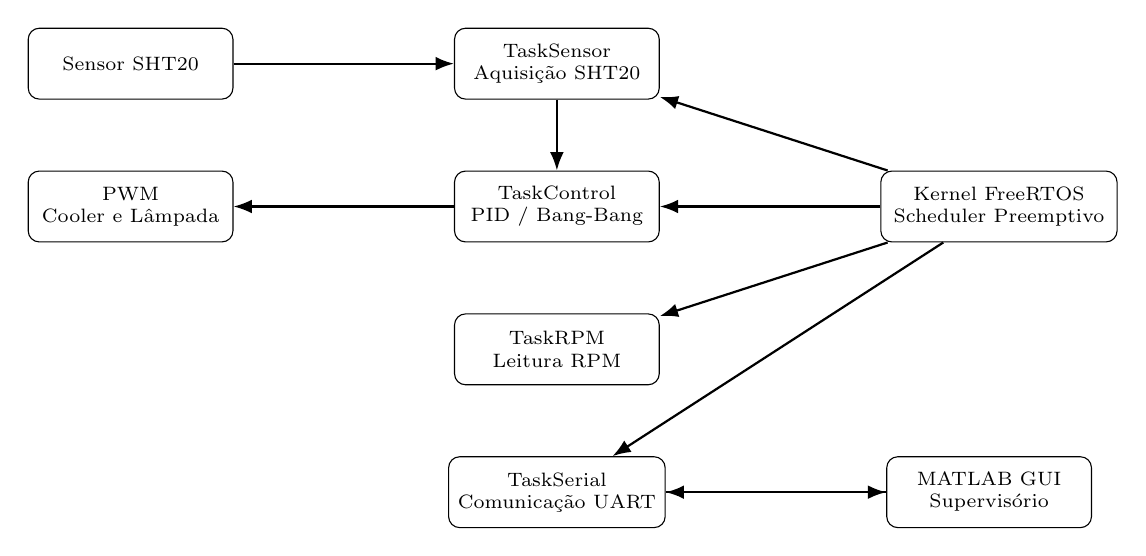
\begin{tikzpicture}[
    node distance=0.9cm and 0.7cm,
    every node/.style={font=\scriptsize},
    bloco/.style={
        draw,
        rounded corners,
        minimum width=2.6cm,
        minimum height=0.9cm,
        align=center
    },
    seta/.style={
        -Latex,
        thick
    }
]

\node[bloco] (sensor) {TaskSensor\\Aquisição SHT20};
\node[bloco, below=of sensor] (control) {TaskControl\\PID / Bang-Bang};
\node[bloco, below=of control] (rpm) {TaskRPM\\Leitura RPM};
\node[bloco, below=of rpm] (serial) {TaskSerial\\Comunicação UART};

\node[bloco, right=2.8cm of control, minimum width=3cm]
    (scheduler) {Kernel FreeRTOS\\Scheduler Preemptivo};

\node[bloco, right=2.8cm of serial] (matlab) {MATLAB GUI\\Supervisório};

\node[bloco, left=2.8cm of control] (atuadores) {PWM\\Cooler e Lâmpada};

\node[bloco, left=2.8cm of sensor] (sht20) {Sensor SHT20};

\draw[seta] (sht20) -- (sensor);
\draw[seta] (sensor) -- (control);
\draw[seta] (control) -- (atuadores);
\draw[seta] (serial) -- (matlab);
\draw[seta] (matlab) -- (serial);
\draw[seta] (scheduler) -- (sensor);
\draw[seta] (scheduler) -- (control);
\draw[seta] (scheduler) -- (rpm);
\draw[seta] (scheduler) -- (serial);

\end{tikzpicture}
}
    \caption{Arquitetura de software multitarefa baseada em FreeRTOS.}
    \label{fig:arquitetura_software}
    \caption*{\footnotesize Fonte: Autor.}
\end{figure}

Na arquitetura proposta, a tarefa \texttt{TaskSensor}
é responsável pela aquisição periódica da temperatura
utilizando o sensor SHT20 via protocolo \IIC{}.
Os dados adquiridos são disponibilizados para a
\texttt{TaskControl}, responsável pela execução do
algoritmo de controle selecionado pelo usuário.

A tarefa de controle realiza o cálculo da ação de controle
com base na estratégia configurada na interface supervisória,
podendo operar em malha aberta, controle bang-bang ou PID.
Após o processamento, os sinais PWM são enviados aos
atuadores da planta térmica, compostos pela lâmpada de
aquecimento e pelo cooler de ventilação.

A \texttt{TaskRPM} executa a leitura periódica da rotação
do cooler a partir dos pulsos provenientes do sensor Hall,
permitindo o monitoramento do sistema de ventilação.

Já a \texttt{TaskSerial} é responsável pela comunicação
serial bidirecional entre o Arduino Nano e a interface
gráfica desenvolvida em MATLAB.
Por meio dessa tarefa são transmitidos os dados de
temperatura, sinal de controle e rotação do cooler,
bem como recebidos parâmetros de configuração do sistema,
como período de amostragem, referência e ganhos do
controlador PID.

O gerenciamento da execução das tarefas é realizado pelo
kernel do FreeRTOS, utilizando escalonamento preemptivo
baseado em prioridades.
As tarefas relacionadas diretamente ao laço de controle
possuem prioridade elevada, garantindo menor latência
e maior previsibilidade temporal durante a execução do
sistema.

% ------------------------------------------------------------
\subsubsection{Configuração da Comunicação Serial Arduino--MATLAB}
% ------------------------------------------------------------
% MELHORIA: subseção preenchida — estava completamente vazia no original

A comunicação entre o Arduino Nano e o MATLAB é estabelecida
por meio do barramento UART com taxa de transmissão de
\textbf{115200\,bps}, 8 bits de dados, sem paridade e um bit
de parada (configuração 8N1). Essa taxa oferece latência
reduzida (aproximadamente 87\,µs por byte) e
compatibilidade garantida com o conversor USB-Serial
integrado à placa (CH340G ou FT232RL).

\paragraph{Protocolo de mensagens.}
As mensagens trocadas entre os dois ambientes seguem o
formato CSV (\textit{Comma-Separated Values}), com campos
separados por vírgula e cada quadro encerrado pelo caractere
de nova linha \texttt{`\textbackslash n'} (LF, 0x0A).
O Arduino envia periodicamente, a cada período de amostragem
$T$, uma linha no formato:

\begin{center}
\texttt{<temperatura>,<controle>,<rpm>\textbackslash n}
\end{center}

onde \texttt{temperatura} é o valor medido em graus Celsius
com uma casa decimal (ex.: \texttt{35.4}), \texttt{controle}
é o ciclo de trabalho PWM expresso em porcentagem inteira
(0 a 100) e \texttt{rpm} é a rotação calculada do cooler em
RPM\@. Exemplo de mensagem enviada pelo Arduino:

\begin{lstlisting}[caption={Exemplo de mensagem CSV enviada pelo Arduino.},
                   label={lst:csv_arduino}]
35.4,72,1450
\end{lstlisting}

O MATLAB transmite comandos ao Arduino sempre que o usuário
altera parâmetros na GUI\@. O formato do pacote de comando é:

\begin{center}
\texttt{<modo>,<referencia>,<Kp>,<Ti>,<Td>,<histerese>,<umax>,<umin>,<T\_ms>\textbackslash n}
\end{center}

onde \texttt{modo} assume os valores inteiros \texttt{0}
(malha aberta), \texttt{1} (bang-bang) ou \texttt{2} (PID).
Os demais campos são valores de ponto flutuante com duas
casas decimais, exceto \texttt{T\_ms}, que é um inteiro
representando o período de amostragem em milissegundos.

\paragraph{Implementação no Arduino.}
No firmware, a \texttt{TaskSerial} utiliza a função
\texttt{Serial.println()} para transmissão e
\texttt{Serial.available()} / \texttt{Serial.readStringUntil('\textbackslash n')}
para recepção. Um mecanismo de verificação de integridade
conta o número de campos separados por vírgula antes de
atualizar as variáveis globais protegidas por mutex,
descartando pacotes malformados. A variável compartilhada
de parâmetros é protegida por um MUTEX do FreeRTOS para
evitar condições de corrida entre \texttt{TaskSerial} e
\texttt{TaskControl}.

\paragraph{Implementação no MATLAB.}
No ambiente MATLAB R2014a, o objeto \texttt{serial} da
\textit{Instrument Control Toolbox} é utilizado para abrir
a porta COM correspondente ao Arduino Nano. A leitura é
realizada por um timer MATLAB configurado com período igual
ao período de amostragem $T$, que dispara o callback de
leitura \texttt{serialReadCallback}. Esse callback executa
\texttt{fgetl(s)} para ler uma linha completa, faz o
\textit{parse} dos campos via \texttt{strsplit} e atualiza
os vetores de dados utilizados para plotagem nos gráficos da
GUI\@. O envio de parâmetros é realizado pelo callback
\texttt{sendParams}, disparado pelos botões e campos de
edição da interface, que formata a string CSV e chama
\texttt{fprintf(s, formato, valores)}.

% ------------------------------------------------------------
\subsection{Implementação dos Algoritmos de Controle}
% ------------------------------------------------------------
% MELHORIA: seção preenchida — estava completamente vazia no original

Os algoritmos de controle são executados exclusivamente
dentro da \texttt{TaskControl}, conforme a estratégia
selecionada pelo usuário via interface supervisória.
A tarefa recebe o valor de temperatura mais recente por
meio de uma variável global protegida por mutex, compartilhada
com a \texttt{TaskSensor}, e atualiza o sinal de controle
nos registradores de PWM ao final de cada ciclo.

\subsubsection{Malha Aberta}

No modo de malha aberta, o sinal de controle é definido
diretamente pelo campo ``Entrada MV'' da GUI, sem realimentação
da temperatura medida. O valor recebido via serial é
convertido diretamente para o ciclo de trabalho PWM e
aplicado à lâmpada de aquecimento:

\begin{lstlisting}[language=C, caption={Pseudocódigo do modo malha aberta.},
                   label={lst:malha_aberta}]
void TaskControl(void *pvParameters) {
    TickType_t xLastWakeTime = xTaskGetTickCount();
    for (;;) {
        /* Leitura segura dos parametros */
        xSemaphoreTake(xParamsMutex, portMAX_DELAY);
        float mv = params.entradaMV;
        xSemaphoreGive(xParamsMutex);

        /* Aplica diretamente no atuador (0-100% -> 0-255) */
        uint8_t pwmVal = (uint8_t)(mv / 100.0f * 255.0f);
        analogWrite(PIN_LAMPADA, pwmVal);

        vTaskDelayUntil(&xLastWakeTime,
                        pdMS_TO_TICKS(params.T_ms));
    }
}
\end{lstlisting}

\subsubsection{Controle Bang-Bang com Histerese}

No modo bang-bang, o atuador é comutado entre potência
máxima e mínima com base no erro em relação ao setpoint,
com uma banda de histerese $\Delta$ para reduzir o
chaveamento excessivo:

\begin{lstlisting}[language=C, caption={Pseudocódigo do controle bang-bang com histerese.},
                   label={lst:bangbang}]
float bangBangControl(float temp, float ref,
                      float histerese,
                      float umax, float umin,
                      float *estadoAnterior) {
    float erro = ref - temp;
    if (erro > histerese / 2.0f)
        *estadoAnterior = umax;
    else if (erro < -histerese / 2.0f)
        *estadoAnterior = umin;
    /* dentro da banda: mantem estado anterior */
    return *estadoAnterior;
}
\end{lstlisting}

\subsubsection{Controlador PID Discreto}

O controlador PID é implementado na forma posicional descrita
pela Equação~\ref{eq:pid_discreto}, com saturação do
sinal de controle nos limites $U_{min}$ e $U_{max}$
configurados pela GUI\@. O mecanismo de \textit{anti-windup}
interrompe a integração quando o sinal de controle atinge
a saturação, evitando o acúmulo ilimitado do termo integral:

\begin{lstlisting}[language=C, caption={Pseudocódigo do controlador PID discreto com anti-windup.},
                   label={lst:pid}]
float pidControl(float temp, float ref,
                 PIDParams_t *p, PIDState_t *s) {
    float e  = ref - temp;
    float dt = p->T_ms / 1000.0f;   /* periodo em segundos */

    /* Termo proporcional */
    float up = p->K * e;

    /* Termo integral com anti-windup */
    if (!s->saturado)
        s->integral += p->K * (dt / p->Ti) * e;

    /* Termo derivativo com filtro de primeira ordem */
    float ud = p->K * (p->Td / dt)
               * (e - s->ePrev) / (1.0f + p->Td/(p->polo*dt));
    s->ePrev = e;

    /* Sinal de controle */
    float u = up + s->integral + ud;

    /* Saturacao */
    s->saturado = (u > p->umax || u < p->umin);
    u = fmaxf(p->umin, fminf(p->umax, u));

    return u;
}
\end{lstlisting}

A conversão do sinal de controle (em volts) para o ciclo de
trabalho PWM (0 a 255) é feita de forma proporcional ao
intervalo $[U_{min},\,U_{max}]$ configurado.


% ============================================================
\chapter{Resultados Preliminares}
\label{cap:resultados_preliminares}
% ============================================================

Este capítulo apresenta os resultados preliminares obtidos
durante o desenvolvimento do trabalho. Nesta etapa, ainda
não foi realizada a implementação completa do firmware no
microcontrolador Arduino Nano, sendo o foco concentrado na
definição da arquitetura multitarefa baseada no FreeRTOS e
no desenvolvimento inicial da interface gráfica supervisória
em MATLAB.

As definições apresentadas servem como base para a etapa
experimental do TCC-II, na qual será realizada a integração
completa entre a planta térmica, o sistema embarcado e a
interface supervisória.

% ------------------------------------------------------------
\section{Definição da Arquitetura Multitarefa}
% ------------------------------------------------------------

A arquitetura de software proposta para o sistema embarcado
foi organizada com base no modelo multitarefa do FreeRTOS,
considerando requisitos típicos de aplicações de controle em
tempo real, como periodicidade determinística, separação de
responsabilidades e priorização de tarefas críticas.

A divisão funcional em tarefas independentes permite reduzir
a complexidade do sistema, melhorar a organização do código
e facilitar futuras expansões da aplicação. Além disso, a
utilização do escalonador preemptivo do FreeRTOS possibilita
garantir que tarefas associadas ao controle da planta tenham
maior prioridade de execução em relação às tarefas de apoio,
como comunicação serial.

O sistema foi inicialmente estruturado em quatro tarefas
principais, apresentadas na
Tabela~\ref{tab:tarefas_preliminares}.

\begin{table}[htbp]
\centering
\caption{Definição preliminar das tarefas do sistema embarcado.}
\label{tab:tarefas_preliminares}
\begin{tabular}{p{3cm} p{2cm} p{2cm} p{7cm}}
\hline
\textbf{Tarefa} &
\textbf{Prioridade} &
\textbf{Período} &
\textbf{Função} \\
\hline

\texttt{TaskSensor} & 3 & $T$ ms &
Realizar a aquisição periódica da temperatura da planta
térmica por meio do sensor SHT20. \\

\texttt{TaskControl} & 3 & $T$ ms &
Executar o algoritmo de controle selecionado
(PID, bang-bang ou malha aberta). \\

\texttt{TaskRPM} & 2 & 1000 ms &
Calcular a rotação do cooler a partir dos pulsos do sensor
Hall. \\

\texttt{TaskSerial} & 1 & $T$ ms &
Realizar a comunicação serial entre o Arduino Nano e o
MATLAB\@. \\

\hline
\end{tabular}
\vspace{0.2cm}
\small Fonte: Autor.
\end{table}

As tarefas \texttt{TaskSensor} e
\texttt{TaskControl} foram definidas com maior prioridade
por estarem diretamente relacionadas ao laço de controle da
planta térmica. Essas tarefas necessitam operar com baixa
latência e periodicidade constante, garantindo que a leitura
da temperatura e o cálculo do sinal de controle ocorram de
forma determinística.

A escolha de períodos idênticos para ambas as tarefas busca
manter sincronismo entre aquisição e atuação, evitando que o
controlador opere com dados desatualizados do processo. O
período de amostragem $T$ será ajustável em tempo real pela
interface supervisória, permitindo avaliar experimentalmente
a influência da taxa de amostragem sobre o desempenho do
controle.

A tarefa \texttt{TaskRPM} foi definida com prioridade
intermediária e período de 1000~ms, uma vez que a medição da
rotação do cooler não interfere diretamente na dinâmica
principal do controle térmico.

Já a \texttt{TaskSerial} recebeu a menor prioridade do
sistema, pois atrasos eventuais na transmissão serial não
comprometem diretamente a estabilidade do controle.

A arquitetura proposta utiliza o escalonamento preemptivo do
FreeRTOS aliado ao mecanismo de atraso periódico
\texttt{vTaskDelayUntil()}, permitindo que as tarefas sejam
executadas com referência absoluta de tempo e reduzindo os
efeitos de \textit{jitter} temporal.

% ------------------------------------------------------------
\section{Interface Gráfica de Supervisão}
\label{sec:gui_preliminar}
% ------------------------------------------------------------

Com o objetivo de facilitar a supervisão da planta térmica e
a interação com o sistema embarcado, foi desenvolvida uma
interface gráfica preliminar em MATLAB R2014a.
A GUI foi implementada de forma programática em um único
arquivo \texttt{.m}, permitindo maior simplicidade de
manutenção e compatibilidade com versões antigas do MATLAB.

A Figura~\ref{fig:gui_hvac} apresenta a proposta inicial da
interface supervisória desenvolvida para o projeto.

\begin{figure}[htbp]
    \centering
    \caption{Interface gráfica preliminar desenvolvida em MATLAB para supervisão da planta térmica HVAC.}
    \label{fig:gui_hvac}
    \includegraphics[width=0.95\textwidth]{figuras/Matlab_ideia_GUI.png}
    \caption*{\footnotesize Fonte: Autor.}
\end{figure}

A interface foi organizada em regiões funcionais destinadas
à conexão serial, configuração dos parâmetros de controle,
visualização das variáveis do processo e exibição gráfica da
resposta do sistema.

Na região superior encontram-se os controles de conexão com
a porta serial do Arduino Nano.
O painel lateral esquerdo reúne os controles de configuração
do experimento e permite selecionar o modo de operação da
planta entre malha aberta, bang-bang e PID.
Além disso, a interface disponibiliza campos para ajuste dos
principais parâmetros do sistema, incluindo período de
amostragem, valor de referência, tensão aplicada ao cooler,
banda de histerese e parâmetros do controlador PID, como
$K_p$, $T_i$ e $T_d$.

Os parâmetros configuráveis da interface estão apresentados
na Tabela~\ref{tab:gui_params}.

\begin{table}[htbp]
  \caption{Parâmetros configuráveis na interface gráfica.}
  \label{tab:gui_params}
  \centering
  \begin{tabular}{lll}
    \hline
    \textbf{Campo} & \textbf{Unidade} & \textbf{Descrição} \\
    \hline
    Tempo ($T$)  & s    & Período de amostragem \\
    Referência   & °C   & \textit{Setpoint} de temperatura \\
    Cooler       & V    & Tensão de perturbação \\
    Histerese    & °C   & Banda do controlador bang-bang \\
    Entrada MV   & V    & Tensão manual em malha aberta \\
    $K_p$        & ---  & Ganho proporcional do PID \\
    $U_{max}$    & V    & Tensão máxima do atuador \\
    $T_i$        & s    & Constante de tempo integral \\
    $U_{min}$    & V    & Tensão mínima do atuador \\
    $T_d$        & s    & Constante de tempo derivativa \\
    Polo $p$     & ---  & Polo do filtro derivativo \\
    \hline
  \end{tabular}
  \caption*{Fonte: Autor.}
\end{table}

% MELHORIA: detalhes de implementação da GUI adicionados
\subsubsection{Estrutura de Implementação da GUI}

O arquivo \texttt{hvac\_gui.m} é estruturado em quatro
blocos funcionais principais:

\begin{enumerate}
    \item \textbf{Inicialização:} a função principal cria a
    janela (\texttt{figure}), instancia todos os controles
    (\texttt{uicontrol}) e inicializa as variáveis de estado,
    incluindo os vetores de dados temporais para plotagem e
    o objeto serial \texttt{s = serial(porta)};

    \item \textbf{Callbacks de conexão:} o botão
    ``Conectar'' dispara \texttt{connectCallback}, que abre
    a porta COM com \texttt{fopen(s)} e cria o timer MATLAB
    (\texttt{t = timer('Period', T, 'ExecutionMode',
    'fixedRate', 'TimerFcn', @serialReadCallback)}), iniciado
    com \texttt{start(t)};

    \item \textbf{Callback de leitura (\texttt{serialReadCallback}):}
    chamado a cada período $T$, executa \texttt{fgetl(s)}
    para ler uma linha CSV, faz o \textit{parse} com
    \texttt{strsplit} e atualiza os vetores de temperatura,
    controle e RPM\@. Em seguida, chama \texttt{set(hLine,
    'YData', dadosTemp)} para atualizar os gráficos sem
    recriar os objetos gráficos (\textit{update-in-place}),
    o que garante desempenho adequado para $T \geq 200$\,ms;

    \item \textbf{Callbacks de envio (\texttt{sendParams}):}
    disparados pelos botões ``Aplicar'' e ``Iniciar'',
    formatam a string CSV de parâmetros e chamam
    \texttt{fprintf(s, '\%s\textbackslash n', csvStr)} para
    transmissão imediata ao Arduino.
\end{enumerate}

A região central superior apresenta indicadores numéricos
para monitoramento das principais variáveis do sistema,
como temperatura medida, valor de referência, sinal de
controle e rotação do cooler.

A região direita da interface contém os gráficos de
monitoramento temporal, responsáveis pela exibição da
temperatura da planta e do sinal de controle ao longo do
tempo.

Nesta etapa do trabalho, a GUI possui caráter preliminar e
tem como principal objetivo validar a organização visual da
interface e a estrutura de supervisão do sistema.
A integração completa com a comunicação serial em tempo real
e com a planta térmica será implementada na etapa seguinte
do projeto.


% ============================================================
\chapter{Proposta de Trabalho}
% ============================================================

% ------------------------------------------------------------
\section{Escopo e Delimitações}
% ------------------------------------------------------------
% MELHORIA: seção preenchida — estava completamente vazia no original

O presente trabalho tem como escopo o desenvolvimento e a
validação de uma arquitetura de controle em tempo real para
a planta térmica didática HVAC da Quanser, utilizando o
FreeRTOS no microcontrolador ATmega328P integrado ao
ambiente de supervisão MATLAB R2014a. O sistema abrange a
implementação do firmware multitarefa, o protocolo de
comunicação serial, os algoritmos de controle (malha aberta,
bang-bang e PID) e a interface gráfica supervisória.

\subsection{Delimitações}

As seguintes atividades e abordagens estão fora do escopo
deste trabalho:

\begin{itemize}
    \item \textbf{Identificação formal da planta:} não será
    realizada identificação paramétrica da função de
    transferência por métodos de mínimos quadrados ou
    equivalentes. A sintonia do controlador PID será
    conduzida por métodos empíricos (Ziegler-Nichols ou
    tentativa e erro supervisionado);

    \item \textbf{Controle em cascata ou multivariável:}
    o trabalho restringe-se a estratégias SISO (\textit{Single
    Input Single Output}), considerando apenas a temperatura
    interna como variável de processo e a lâmpada de
    aquecimento como atuador principal;

    \item \textbf{Controle adaptativo ou preditivo:} não
    serão implementados algoritmos com ajuste automático de
    parâmetros (auto-tuning) ou com modelo interno de predição
    (MPC);

    \item \textbf{Outras plataformas de hardware:} o sistema
    será desenvolvido exclusivamente para o Arduino Nano
    (ATmega328P). Portabilidade para outras plataformas
    (STM32, ESP32, etc.) não está prevista neste trabalho;

    \item \textbf{Comunicação sem fio:} a integração
    Arduino--MATLAB será realizada exclusivamente via
    interface serial cabeada (USB-UART). Protocolos sem fio
    (Wi-Fi, Bluetooth, MQTT) estão fora do escopo;

    \item \textbf{Interface MATLAB Simulink ou modo externo:}
    a supervisão será realizada por GUI programática em
    MATLAB puro (\texttt{.m}), sem o uso de modelos Simulink
    ou da infraestrutura de geração automática de código.
\end{itemize}

\subsection{Contribuições Esperadas}

Ao final do TCC-II, espera-se entregar as seguintes
contribuições concretas:

\begin{itemize}
    \item \textbf{Firmware documentado:} código-fonte
    completo do sistema embarcado, organizado segundo a
    arquitetura multitarefa proposta, com comentários e
    instruções de compilação no ambiente Arduino IDE com a
    biblioteca FreeRTOS-AVR;

    \item \textbf{Interface gráfica funcional:} arquivo
    \texttt{hvac\_gui.m} funcional no MATLAB R2014a, com
    comunicação serial bidirecional operacional, exibição
    gráfica em tempo real e controle dos modos de operação
    da planta;

    \item \textbf{Dados experimentais:} conjuntos de dados
    de resposta ao degrau e de rejeição a distúrbios para
    as estratégias bang-bang e PID, coletados em condições
    reprodutíveis e armazenados em formato \texttt{.csv}
    para análise posterior;

    \item \textbf{Análise comparativa:} avaliação
    quantitativa do desempenho dos controladores (tempo de
    subida, sobressinal, tempo de acomodação, erro em regime
    permanente e \textit{jitter} de amostragem) e da
    influência do período de amostragem $T$ sobre a
    estabilidade e a precisão do controle.
\end{itemize}


% ============================================================
\chapter{Cronograma de Atividades}
% ============================================================

O cronograma de atividades previsto para a conclusão deste trabalho está apresentado no \autoref{quad:cronograma}. As atividades estão distribuídas ao longo do segundo semestre de 2026, contemplando a finalização da implementação, a realização dos experimentos, a análise dos resultados e a redação do documento final.

\begin{quadro}[htb]
\caption{Cronograma de atividades para o segundo semestre de 2026.}
\label{quad:cronograma}
\centering
\begin{tabular}{lccccc}
\hline
\textbf{Atividade} & \textbf{Ago} & \textbf{Set} & \textbf{Out} & \textbf{Nov} & \textbf{Dez} \\
\hline
Revisão bibliográfica complementar          & $\bullet$ & $\bullet$ &           &           &           \\
Sintonia experimental do controlador PID    & $\bullet$ & $\bullet$ &           &           &           \\
Validação experimental (resposta ao degrau) &           & $\bullet$ & $\bullet$ &           &           \\
Validação (rejeição a distúrbios)           &           &           & $\bullet$ &           &           \\
Análise comparativa PID vs.\ bang-bang      &           &           & $\bullet$ & $\bullet$ &           \\
Redação dos capítulos de resultados         &           &           & $\bullet$ & $\bullet$ &           \\
Redação das considerações finais            &           &           &           & $\bullet$ & $\bullet$ \\
Revisão geral e formatação                  &           &           &           & $\bullet$ & $\bullet$ \\
Entrega e defesa do TCC                     &           &           &           &           & $\bullet$ \\
\hline
\end{tabular}
\fonte{Autor.}
\end{quadro}


\printbibliography

\end{document}
